\begin{figure}[t!]
\centering
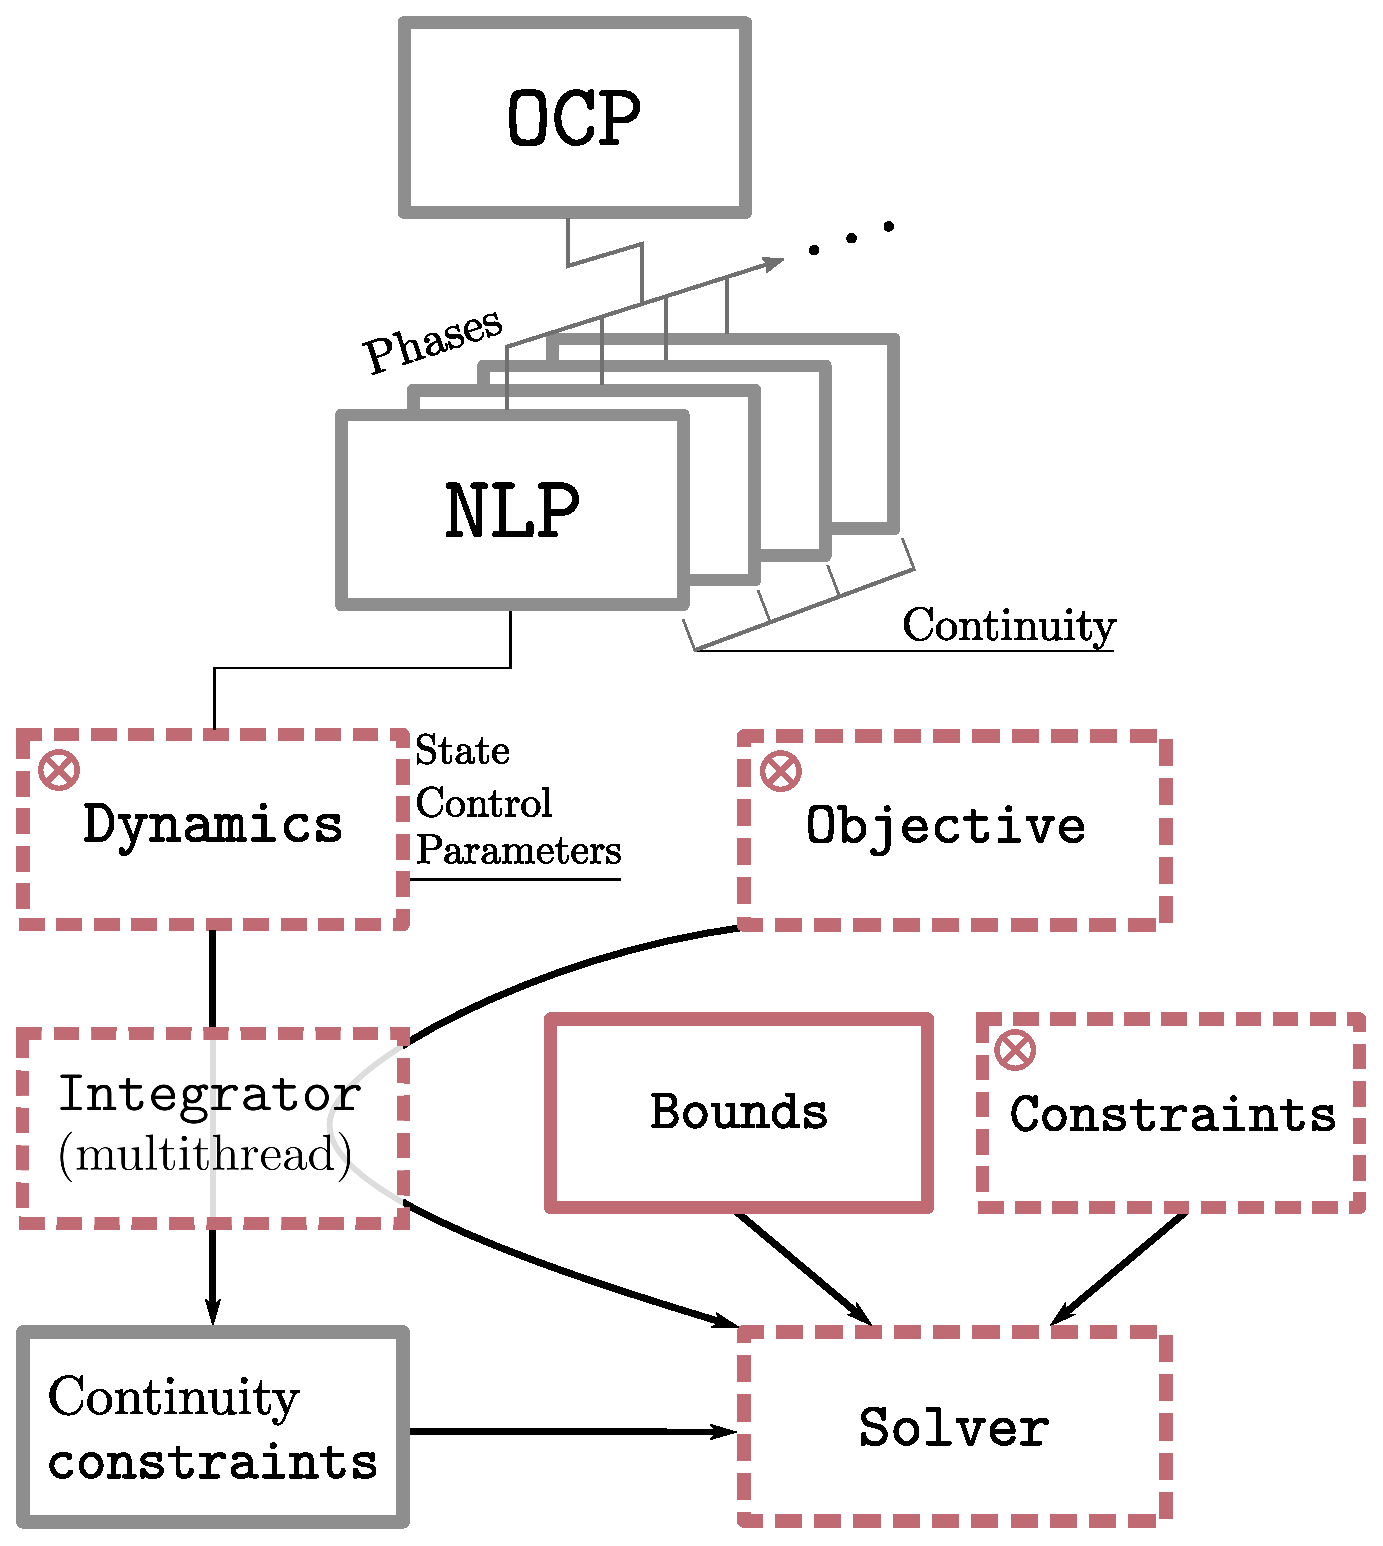
\includegraphics[width=0.9\columnwidth]{figures/design.eps}
\caption{\bioptim design flowchart. The red box correspond to objects that must be filled in by the user. The red-dashed boxes correspond to pre-implemented objects already available to the users. $\otimes$ stands for easily customizable objects.}
\label{fig:flowchart}
\vspace*{-0.5cm}
\end{figure}
\subsection{Implementation and dependencies}
\bioptim is the top layer of a series of libraries (\biorbd: dynamics and MSK modeling; \casadi: automatic differentiation; \ipopt/\acados: optimization; \bioviz: visualization).
Within this software suite, \bioptim 's main role is to shape the problem to allow its dependencies to communicate efficiently, while providing an intuitive and flexible interface to the user (Fig.~\ref{fig:dependencies}).
Therefore, it was written in Python for its flexibility and its widespread use among researchers.
However, all intensive calculations behind the interface are performed in C/C++, keeping \bioptim both fast and easy to customize.

\subsection{Design}
\bioptim shapes and solves optimal control problems whose two required entries are a model (.\textit{bioMod} file) and an OCP.
The model file contains the geometrical characteristics and the segment inertial parameters as well as optional elements, namely, the markers, the actuators of the model (muscles and joint torques possibly with torque/angle/velocity relationships) as well as bounds on joint kinematics and torques. 
It also allows the user to design or import meshes for visualization purposes.
The \texttt{OCP} consists in a combination of nonlinear problems (NLPs) that allows for the formulation of multi-staged OCPs. 
Each \texttt{NLP} has the following attributes: \textit{1)} a dynamics type, \textit{2)} an objective function set, \textit{3)} a constraint set, \textit{4)} variables bounds, \textit{5)} a number of shooting points and the duration of the problem and \textit{6)} initial guesses.
Based on these inputs, \bioptim properly sets up the multiple shooting transcription of the OCP, with appropriate continuity constraints (between the shooting nodes and the phases) and shapes it up to feed the chosen nonlinear solver (\ipopt or \acados). 
Next, we develop the different attributes of each \texttt{NLP}:

\subsubsection{Dynamics}
The dynamics defines which variables are states ($\state$), controls ($\control$) and parameters ($\param$), the latter being time-independent.
Then, it implements the ordinary differential equation governing the state dynamics:

\[
\dstate = f(\state, \control, \param).
\addtag
\label{eq:state_transition}
\]

\noindent More than 10 dynamics are already implemented in \bioptim, among which the controls (piecewise constant or linear) can be muscle excitations, muscle activations and/or joint torques, the states can be muscle activations and/or joint kinematics.
They can include contact points, external forces, etc.
Even if these dynamics types exhaustively span the current usages in biomechanics, a custom dynamics type is also pre-implemented to easily customize problems.

\subsubsection{Objective function set}
In line with the optimal control formalism, there are two main types of objective functions, namely Lagrange and Mayer. 
Lagrange types are running objectives, integrated over the NLP duration. Mayer types are time-specific objectives. 
Classically, they correspond to a terminal objective, but to be more versatile, they can be defined at any instant in \bioptim.

\objectives can depend on any of the optimization variables, \textit{i.e.} the controls, the states, the parameters and the duration of the problem. 
A lot of objective function types are already implemented in \bioptim ($>\negmedspace 20$), among which tracking\:/\:minimizing, on states\:/\:controls\:/\:markers\:/\:contact\:forces\:/\:problem\:duration, etc. 
Should one go missing, a custom objective type is also possible to define.

When declaring the desired list of objective functions for a given NLP, each objective function type is associated with a weight, and the user can choose on which components of the vector variables the objective must apply. 
If applicable (for tracking objective functions mainly), the user must also specify the numerical target of the objective.

\subsubsection{Constraint set}
Classically, constraints are hard penalties of the optimization problem, i.e., a solution will not be considered optimal, unless all constraints (equality or inequality) are met.
The \texttt{Constraint} class contains a variety of implemented constraints.
Some of them are specific functions, commonly useful in biomechanical problems (e.g. non-slipping contact point, non-linear bounds on torque depending on the state, etc.), the others have their equivalent in the \texttt{ObjectiveFunction} class.
Should one go missing, a custom constraint type is also possible to define.

\subsubsection{Bounds}
Essentially, the \texttt{Bounds} are constraints directly related to the states, the controls and the parameters.
They are useful to define model-related constraints such as kinematic, torque or muscle excitation\:/\:activation limits. 

\subsubsection{Shooting points and problem duration}
In direct multiple shooting, the total duration of the problem is divided into smaller intervals whose initial values are called shooting points. 
In \bioptim, the user is asked to define a number of shooting points and a problem duration, per phase.
Possibly, the problem duration can be part of the optimization variables, allowing for, e.g., minimal time formulations.

\begin{figure}[t!]
\centering
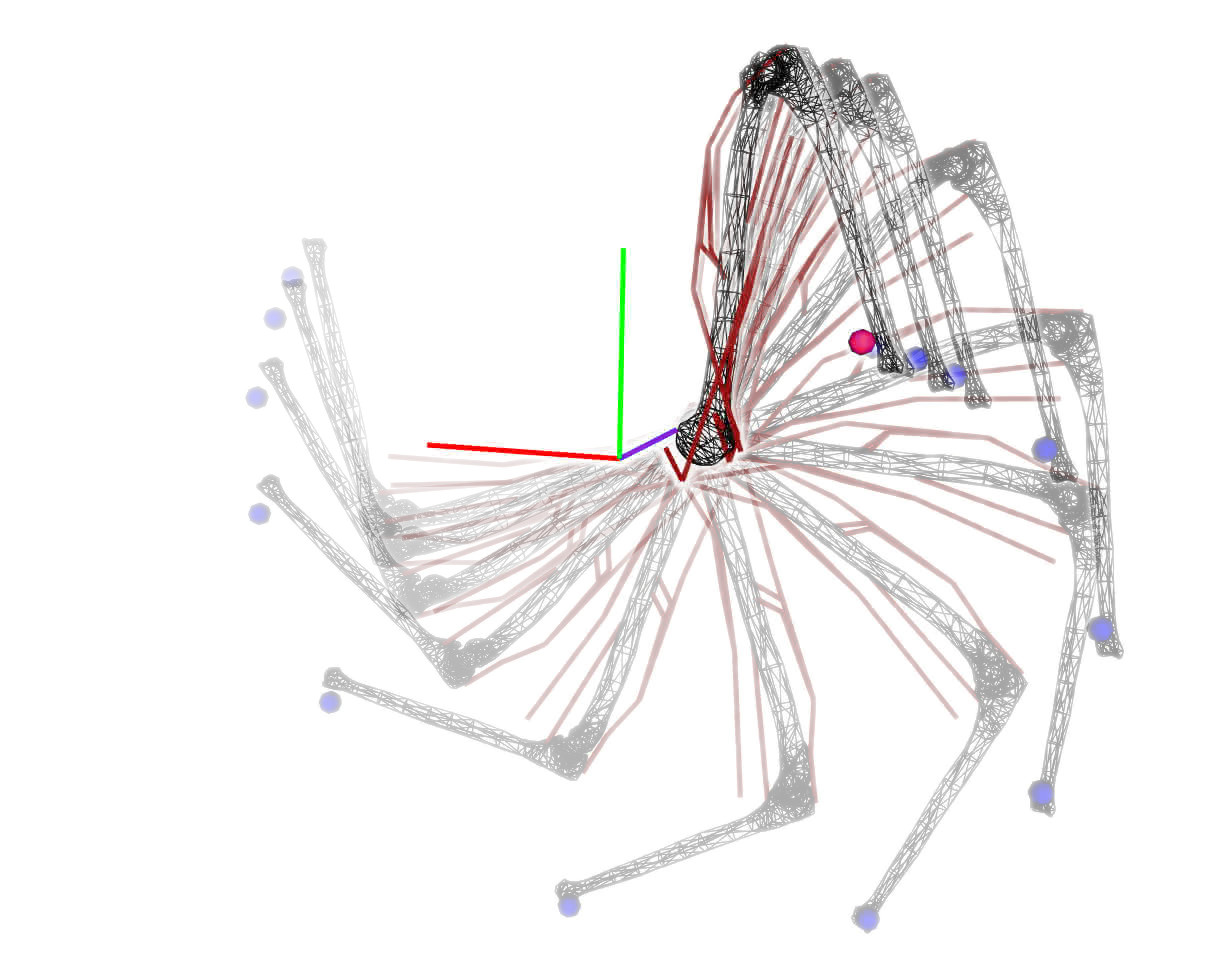
\includegraphics[width=\columnwidth]{figures/activation_pointing.jpeg}\\
\caption{Snapshots of an optimized activation-driven pointing task with \acados. The arm starts facing upwards in left hand part of the picture and ends facing downwards in the right hand part. The marker fixed on the ulna head is depicted in blue and the scene-fixed target marker is depicted in red. Red lines show the lines of actions of the muscles.}
\label{fig:snapshots_activation_driven_pointing}
\vspace*{-0.5cm}
\end{figure}
\subsubsection{Initial guesses}
The user can provide an \texttt{InitialGuess} for all the optimization variables, at each shooting point.
This feature aims at providing prior information to the solver.
Several \texttt{InterpolationTypes} are implemented (constant, linear, spline, each point, etc.), to quickly let the user define the initial guesses.
A custom \texttt{InterpolationType} is also possible to implement.
\begin{figure*}[t!]
\centering
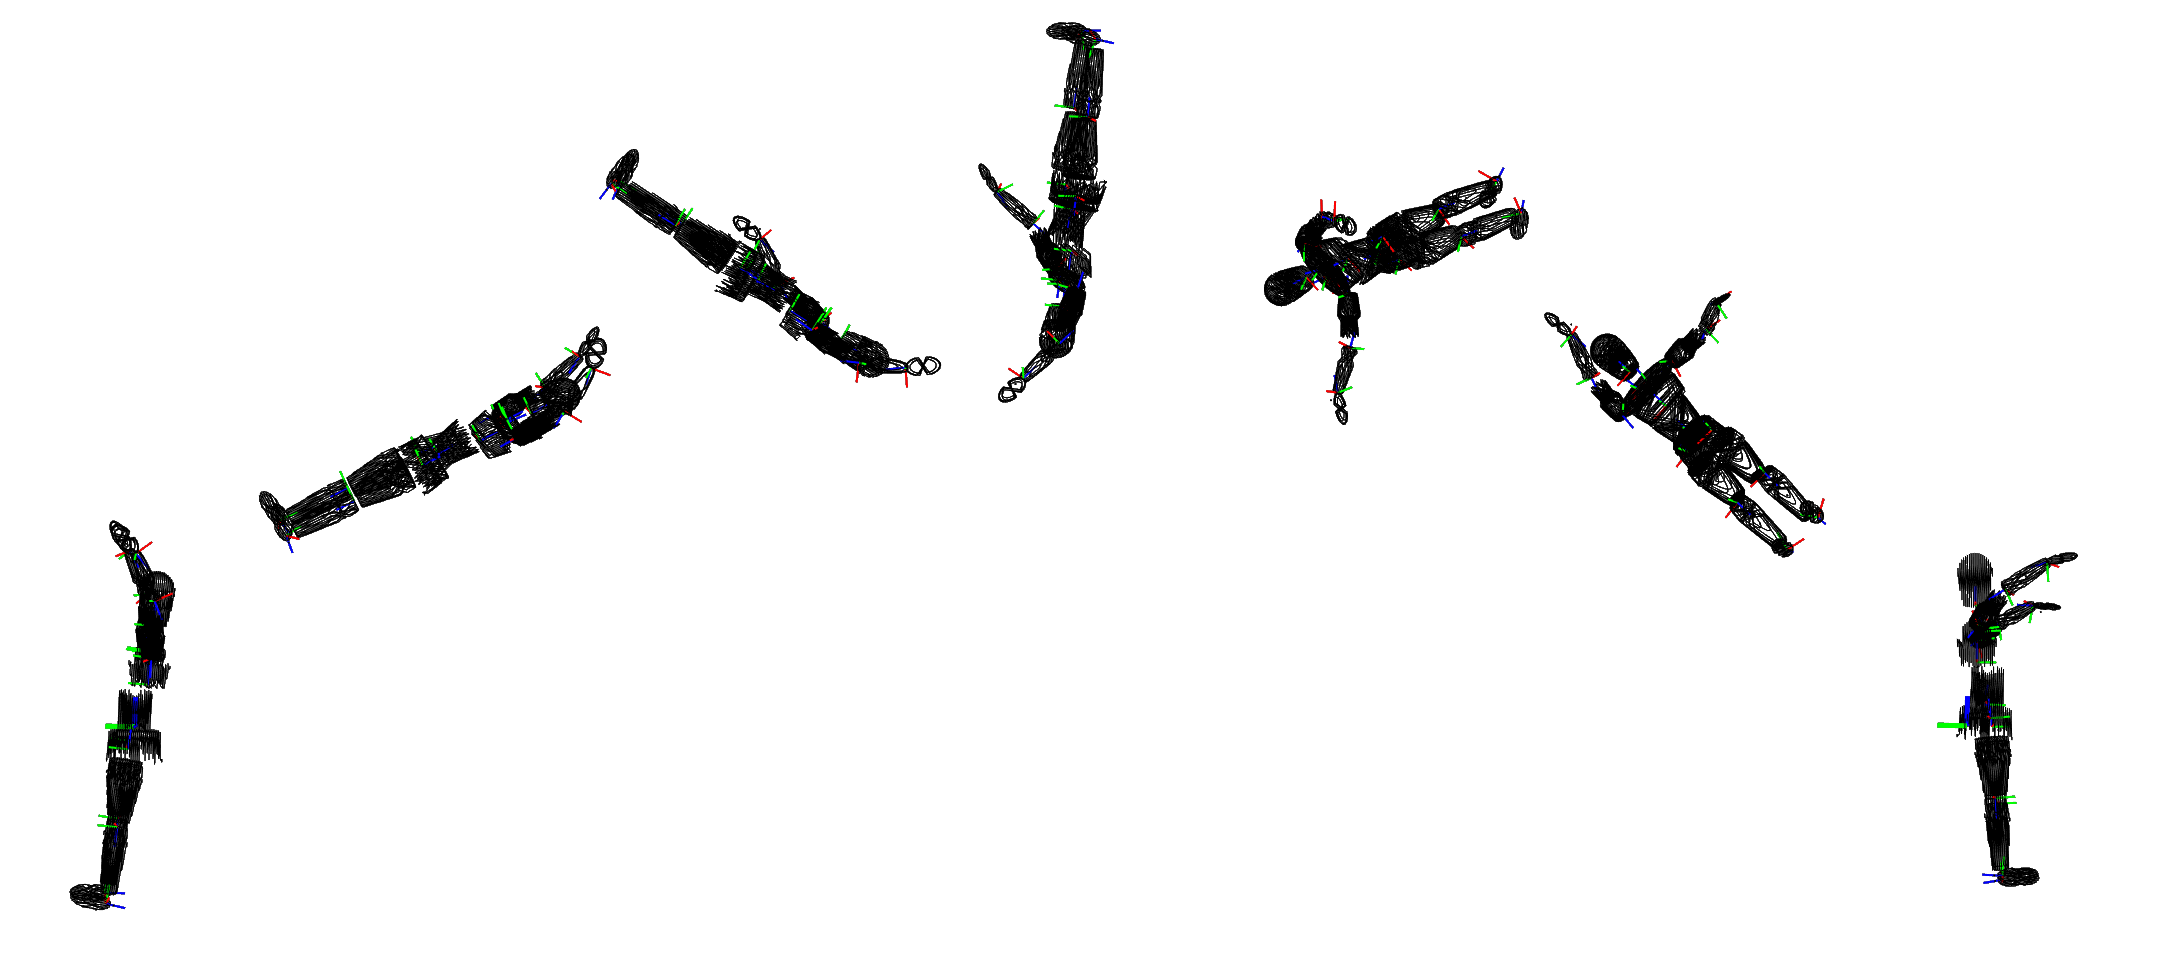
\includegraphics[width=\textwidth]{figures/Euler_Bioptim_MaxVrille_dos_7frames.png}
\caption{Snapshots of maximally twisting somersaults driven by shoulder torque actuators and a free base whose rotation is either expressed by Euler angles (top) or by quaternions (bottom).}
\label{fig:snapshots_quaternion_base_twisting_somersault}
\end{figure*}